\section{Referências Bibliográficas}

\begin{frame}{Referências Bibliográficas}
A forma mais simples de se referenciar dentro de um texto é usando o ambiente {\ttfamily thebibliography}.
\lstinputlisting{citacoes/std.tex}
\end{frame}

\begin{frame}{O Bib\TeX{}}
Entretanto, o Bib\TeX{} é uma ferramenta que oferece muito mais flexibilidade na formatação dos textos\footnote{Incluir o pacote \textit{natbib} para gerenciar os recursos do Bib\TeX{}.}.
\lstinputlisting{citacoes/biblio.tex}
Alguns dos estilos de bibliografia são esses:
\begin{enumerate}
	\item IEEEtran
	\item abnt-num
	\item abnt-alf
	\item sbc
	\item apalike
	\
\end{enumerate}
\end{frame}

\begin{frame}[fragile]
\begin{lstlisting}[linewidth=10cm]
@inproceedings{praciano2018spatio,
  title={Spatio-Temporal Trend Analysis of the Brazilian Elections Based on Twitter Data},
  author={Praciano, Bruno Justino Garcia and da Costa, Jo{\~a}o Paulo Carvalho Lustosa and Maranh{\~a}o, Jo{\~a}o Paulo Abreu and de Mendon{\c{c}}a, F{\'a}bio L{\'u}cio Lopes and de Sousa J{\'u}nior, Rafael Timoteo and Prettz, Juliano Barbosa},
  booktitle={2018 IEEE International Conference on Data Mining Workshops (ICDMW)},
  pages={1355--1360},
  year={2018},
  organization={IEEE}
}
\end{lstlisting}
\end{frame}

\begin{frame}
Uma lista de tipos de referências, com todas suas entradas possível, pode ser acessada pelo link:
\begin{center}
\url{https://en.wikibooks.org/wiki/LaTeX/Bibliography_Management}
\end{center}
\end{frame}

\subsection*{Coletando citações}

\begin{frame}{Use o \href{http://scholar.google.com.br}{Google Acadêmico}}
	
\begin{figure}[htbp!]
	\centering
	\includegraphics[width=0.6\textwidth]{figuras/google1.png}
	\caption{ }
\end{figure}
\end{frame}

\begin{frame}{Coletando citações}
	
\begin{multicols}{2}
\begin{figure}[htbp!]
	% \centering
	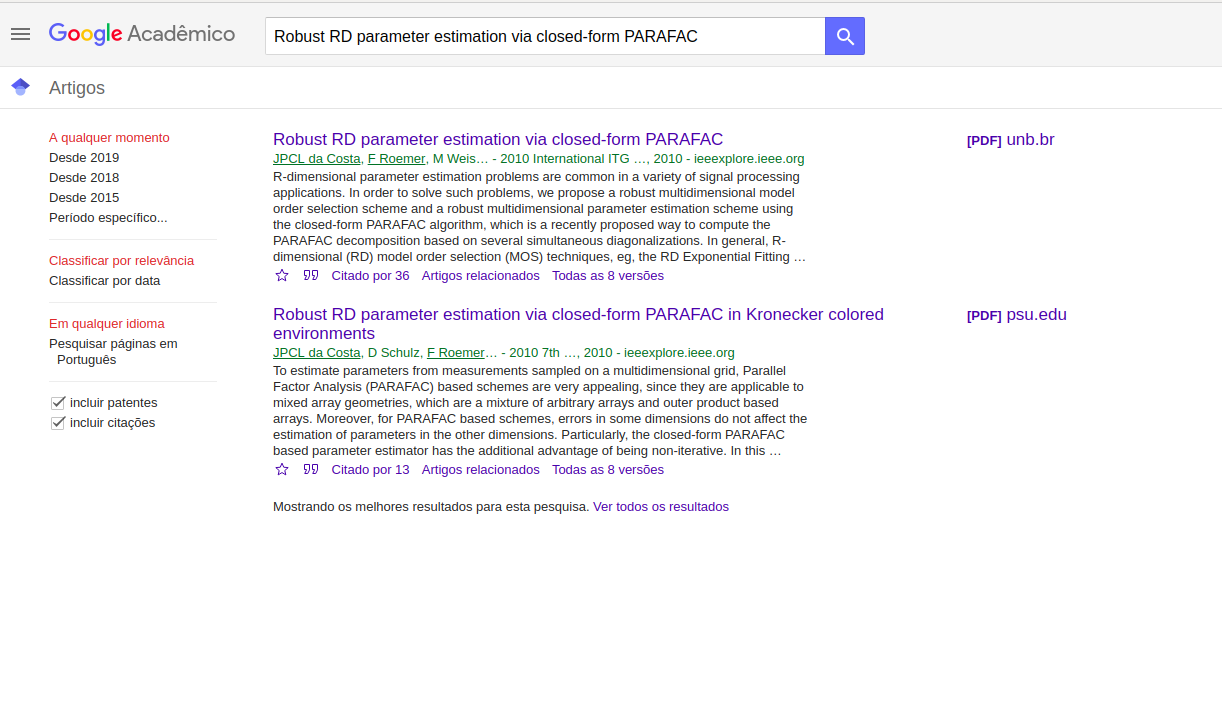
\includegraphics[width=0.6\textwidth]{figuras/google2.png}
	\caption{ }
\end{figure}
	
\begin{figure}[htbp!]
	\centering
	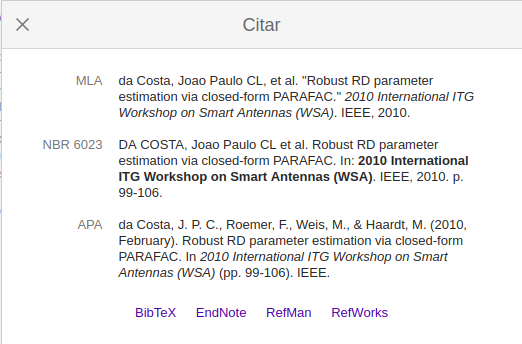
\includegraphics[width=0.4\textwidth]{figuras/google3.png}
	\caption{ }
\end{figure}
\end{multicols}
\end{frame}
	

